\chapter{Data Description}
\label{chap:ddesc}

This section depicts the datasets provided by the project’s industrial partners. We give an overview on a retailer and on fashion-tech startup potential datasets. We will also describe the datasets content and focus on their future use in the context of FashionBrain. This section will be briefly extended by introducing the data integration technique that will be deployed. Table~\ref{tab:data-zalando} summarizes the main properties of the datasets provided by Zalando.
\smallskip


\begin{table}[htb]\centering
\def\arraystretch{1.2}
\begin{tabular}{|l|c|c|l|c|}
\hline
 \textbf{File name} & \textbf{Format}  &  \textbf{Size} & \textbf{Brief description} & \textbf{Date} \\
 \hline\hline
 region1\_items & csv  &22.2 MB  &Items classification in Zalando &  31.03.2017  \\
 region2\_items &  &  &anonymized tree with the & \\
 &  &  & amount and \# of items sold  &  \\
 \hline
 region1\_orders & csv  &42 KB  &Items’ orders with the gross  &  31.03.2017  \\
 region2\_orders &  &  &amount  & \\
 \hline
zalando-images- & csv  &1.01 GB  &A detailed identification of  &  24.04.2017  \\
attributes-FB- &  &  &products from different brands& \\
release&  &  & and their specialized features  &  \\
 \hline
zalando-reviews- & csv  &355.2 MB  &Users’ comments on different  &  24.04.2017  \\
FB-release&  &  & products& \\
 \hline
OEM\_ & csv  &5.2 MB  &Mapping of item attributes &  31.03.2017  \\
translations&  &  & rendered in different  & \\
&  &  &  languages on the web site & \\
 \hline
\end{tabular}
\caption{Datasets provided by Zalando.}
\label{tab:data-zalando}
\end{table}
\smallskip

Table~\ref{tab:data-fashwell} summarizes the main properties of the datasets provided by Fashwell.

\begin{table}[htb]\centering
\def\arraystretch{1.2}
\begin{tabular}{|l|c|c|l|c|}
\hline
 \textbf{File name} & \textbf{Format}  &  \textbf{Size} & \textbf{Brief description} & \textbf{Date} \\
 \hline\hline
dump-example- & json &3.6 MB  &A detailed identification of&  30.03.2017  \\
macys &  &  &  products   from “Macys” with & \\
 &  &  &  their specialized features & \\
\hline 
dump-example- & json & 4.3 MB  &A detailed identification of  &  30.03.2017  \\
gap &  &  & products from “GAP” with & \\
 &  &  & their specialized features & \\
\hline 
products-example & json &512 KB &an example of the json  &  30.03.2017  \\
 &  &  & description of a given product  & \\
\hline 
fashion\_tree\_dump& csv &21 KB  &Fashwell Fashion tree  &  04.05.2017  \\
\hline 
products-schema & json &3 KB  &A schema explaining  &  30.03.2017  \\
 &  &  &  the content of the json files  & \\
\hline 
\end{tabular}
\caption{Datasets provided by Fashwell.}
\label{tab:data-fashwell}
\end{table}

\section{Fashion Retailer Data}

This section provides a detailed description of the datasets provided by Zalando and that will be used in order to offer exclusive data services to their customers as they will be able to  anticipate customer needs, and predict short and long term trends or frauds. The datasets are in the form of csv files containing each a table of attributes.  This section will be divided into two parts. In the first part, the attributes of each file will be presented by providing their type and description. Next, we will analyse how these datasets can be used in terms of research. In the second part, we will summarize the relationship between the files in a relational schema.

\subsection{Datasets Analysis}

\paragraph*{OEM\_Translation.csv}: In order to keep a tight relation with its clients, Zalando offers the possibility for users to see product attributes in their own language depending on the localization of the website. The OEM\_Translation file includes items’ attributes rendered in different languages on the website. This file is used to map multilingual description to one fashion vocabulary.

\begin{itemize}
    \item Attribute\_type (String): It can be the item’s color, color family or fabric. It can also give an indication about the appropriate season for the item. 
    \item Attribute\_id (String): It gives a unique attribute identifier up to translation i.e. there are multiple instances of each attribute, but their translations have similar meaning in different languages. 	
    \item Language (String): It can be French, English, German, Italian, etc.
    \item Translation (String): It is the translation of the attribute in the indicated Language.
    
\end{itemize}




\paragraph*{Region*\_item.csv (* is either  1 or 2)}: The items dataset splits sales into categories, 
subcategories and sub-subcategories as well as the item’s season (category-level 1-3).

\begin{itemize}
    \item Date (String): The date when an item was sold. The date ranges from March 2013 to March 2015.
    \item Category\_level 1,2,3 (Integer): This is the categorization of items in the Zalando category hierarchy. Example: A long dress could be under clothing, women, dress category. The mapping for ``clothing" could be found in the first category with an id=0 for instance. The mapping for "women" could be found in the second category with an id=1 and ``dress" could be found under the third category with an id =11. In this case, the long dress would be under the 0,1,11 category. The real values are anonymized and they provided values are given for the sake of illustration. \item Season (String): This attribute represents the clothing season for the item e.g., spring/ summer, autumn/ winter, no-season.
    \item Gross\_amount (Float): This attribute represents the amount spent in total normalized by the mean over the column (anonymised revenue value)
    \item No\_items (Float) No of items bought normalized by the mean over the column no\_items could be less or larger than the revenue. It actually depends on the item itself. In fact, selling a lot of socks can generate less revenue than selling a much smaller quantity of suits.
\end{itemize}

\paragraph*{Region*\_orders (* is either  1 or 2)}: A fashion retailer keeps track of item’s orders that it can have a better handle on stock levels. This data was provided in the form of two files Region*\_item and Region*\_orders where * could be 1 or 2 corresponding to two regions where deliveries were made from 2013 until 2015. This data will be used in the prediction package (WP5) where we propose to help retailers to estimate their needed stock. More specifically, we will use the data for the following tasks: i) Prediction of the category with the largest revenue and ii) Prediction of the orders amount on a specific category.

\begin{itemize}
    \item No\_items (Float) Number of items bought normalized by the mean over the column
    \item No\_orders (Float): Number of orders placed normalized by the mean over the column
    \item Gross\_amount (Float): Amount spent in total normalized by the mean over the column
    \item Date (Float):  Date when the order was made. It varies between March 2013 and March 2015
\end{itemize}

\paragraph*{zalando-reviews-FB-release.csv}: Comments and reviews are increasingly important part of the purchase journey for online consumers. Fashion retailers need to take full advantage of this important source of feedback and adjust their offers according to customer’s desires. The file “zalando-reviews-FB-release.csv” contains user’s feedback on purchased items through Zalando website. The data extracted from this file will be part of the input of the Aspect-Oriented Opinion Mining and Entity Linkage packages. For example, some items are very well appreciated by users while in other cases, some items may not match their taste or their idea about them. Thus, research in this area could lead to a deep understanding of consumer’s preferences and subsequently improve the consumer’s online shopping experience.

\begin{itemize}
    \item Title (String): This could be interpreted as the summary of the user’s comment. 
    \item Text (String):  This is the user’s comment in its original language.
    \item sku (String): This is the stock keeping unit, it enables the identification of one specific item.
    \item Language\_Code (String): Here we have two-letter language code which is the original language of the comment.
\end{itemize}

\paragraph*{zalando-images-attributes-FB-release.csv}: This file includes a detailed identification of products from different brands with their specialized features. This file is the one that will be used as a reference to identify the items and extract their specialized features.

\begin{itemize}
    \item As\_sku (String): This is the stock keeping unit, it enables the identification of one specific item.
    \item M\_path (String): Image paths, separated by spaces where each image path needs to be appended to the URL: \url{https//mosaic01.ztat.net/vgs/media/pdp-gallery/)}
    \item  Article\_name (String): Name of the product
    \item Brand\_name (String): Name of the brand
    \item Pool\_name (String): Name of the category
    \item Subpool\_name (String): Name of the subcategory
    \item Main\_color (String):  Name of the main color
    \item Additional\_attributes (JSON key-value pairs): Additional attributes as JSON key-value pairs (each article may have any number of additional attributes)
\end{itemize}

\subsection{Relational Schema}

The relational schema of Figure~\ref{fig:model_rs} describes the relationships between the files  above-mentioned, and provides a comprehensive view of our database. Note that Region*\_items and Region*\_orders are related since the item specification in terms of categorization, season and gross amount is found in the first file while in the second one, we find the number of ordered items per date. Each review is identified by the product SKU which can be recognized with the image-attributes file. Some specific features named in the latter (color, material, etc.) can be translated into other languages with the OEM\_translation file. 



\begin{figure}[htb] \centering 
  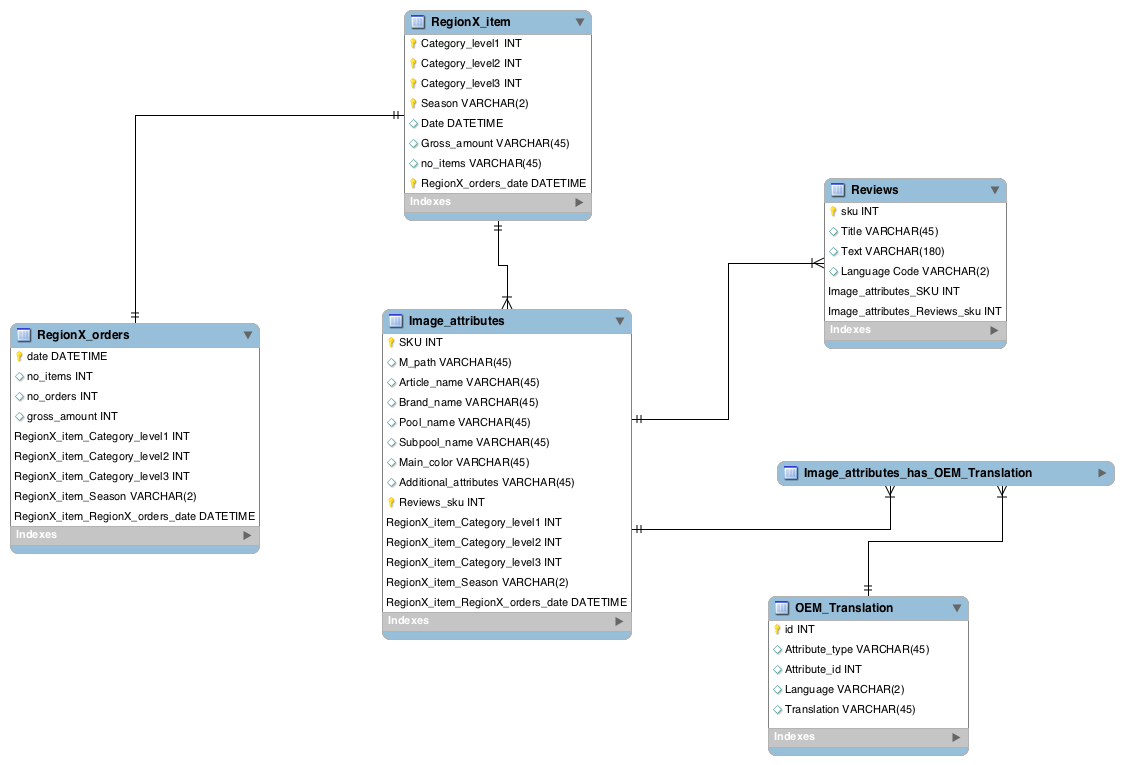
\includegraphics[scale=0.4]{Zalando_RS}
  \caption{Relational model.}
  \label{fig:model_rs}
\end{figure}

%%%%%%%%%%%%%%%%%%%%%%%%%%%%%%%%%%%%%%%%%%%%%%%%%%%%%%%%%%%%%%%%%%%%%%%%%%%%%%%%%%%%%%%%%%%%%%%%%%%%%
%%%%%%%%%%%%%%%%%%%%%%%%%%%%%%%%%%%%%%%%%%%%%%%%%%%%%%%%%%%%%%%%%%%%%%%%%%%%%%%%%%%%%%%%%%%%%%%%%%%%%
\section{Fashion-tech startup}

This section provides an overview of the datasets provided so far by Fashwell. The datasets are in the form of json and csv files. These files are a sample of the data that will be provided by Fashwell. The json files contain brand’s catalogue while the csv files contain a fashion taxonomy. This taxonomy is a fine grained tree of fashion items depending on the gender. We propose to analyse the provided files in order to extract their potential use in terms of research. For the json files, we describe the main attributes and their type. The fashion taxonomy file contains a table of attributes. We describe the most relevant attributes with their respective types. 
We begin by describing two example json files. Each file describes respectively GAP and MACYS online store’s catalogue joined with a schema and an example. These attributes help to extract the product specification, e.g., the categorization of the items will be used in order to build a taxonomy in (WP1).

\paragraph*{dump-example-*.json (* can be GAP or MACYS)}:

\begin{itemize}
    \item Brand (String): Name of Brand
    \item Category (Array of Strings): A categorization hierarchy of the item
    \item Gender (\quotes{enum}: [ \quotes{unisex}, \quotes{female},  \quotes{male}, \quotes{boy}, \quotes{girl}, \quotes{infant}, \quotes{unknown} ]): It could be unisex, female, male, boy, girl, infant or unknown 
    \item Name (String) Name of the item
    \item Internal\_id (String): Internal Order Number
    \item Product\_url (String): Link to the product in the website
    \item Images\_url (Array of Strings): Link to the product image
    \item Desc (String) Gives a description of a product
\end{itemize}

Below we give an example of the json description of one product.

\begin{verbatim}
{ "name": "Nike SB Stefan Janoski Max",
"desc": "The Nike SB Stefan Janoski Max is designed with ...", 
"price": 140.00,			
"msrp": 210.00,
"currency": "EUR",
"sizes": ["34", "38", "40"],
"category": ["men", "accessories", "glasses"],
"images_url": ["http://www.foo.com/bar0.jpg", "http://www.foo.com/bar0.jpg"], 
"gender": "male", "brand": "Nike",
"product_url": "https://www.foo.com/bar/baz",
"ean": 123456789,
"internal_id": "999111",
"features": "110% cotton",
"color": "tomato"
}
\end{verbatim}


Fashwell has different sources of data. In order to have one unique dataset with non redundant elements, they integrate them all together to get one unique fashion tree using the model described in Figure~\ref{fig:classifier}.


\begin{figure}[htb] \centering 
  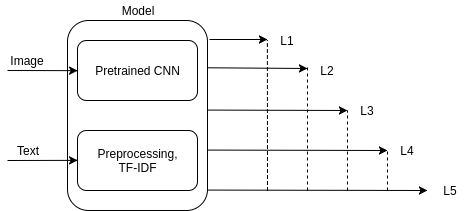
\includegraphics[scale=0.6]{taxonomy_classifier}
  \caption{Fashion items classifier.}
  \label{fig:classifier}
\end{figure}


We provide in what follows a brief description of the model used by Fashwell. This model takes as an input an image and a text associated with one product. For the vision part of the model, a convolutional neural network is used. the model is pre-trained on ImageNet dataset and then fine-tuned to fashion products taxonomy task. The text part of the model uses some NLP techniques for preprocessing, like stemming and stop-word removal, and then uses TF-IDF for feature extraction from the text. In the end, these two parts of the model (vision and text) are combined in a single neural network model which can predict a taxonomy. Interesting finding was that, in most cases, text was much more informative for inferring taxonomy correctly than an image. When a product has multiple images, the classifier is applied on all images with the text describing the product. In a later step, predictions average is made, which usually leads to better results. If there are multiple images per product, the vision part of the model improves in prediction accuracy. This model learns 5 tasks in joint - for each level of taxonomy. The higher the level, the more fine-grained the classification is. It is also taken into consideration the information from the lower levels of predictions to enhance the predictions of higher levels, but still the higher the level, the more imprecise the predictions are. Products with already-labeled taxonomies were used to train the classifier. 

The main attributes of the fashion tree are depicted as follows:

\paragraph*{fashion\_tree\_dump.csv}:

\begin{itemize}
    \item id (Integer): Category id in the Fashwell tree
    \item name (String): Name of the category
    \item parent\_id (Integer): The parents id of a particular category. 
    \item gender (enum: [ \quotes{unisex}, \quotes{female},  \quotes{male}, \quotes{boy}, \quotes{girl},\quotes{infant}, \quotes{unknown} ]): The gender could be any element of the enum set
\end{itemize}

In the following section, we describe the results of the survey on how social media influences the shopping experience of their viewers. This survey aims to help us discovering the platforms and the fashion blogs that are used as fashion drivers. 

